% =========================
% sections/device_process.tex
% =========================
\section{Device and Process Integration}

\subsection{LPDDR Technology Background}
Low-power DRAM (LPDDR) is the de-facto main memory for mobile systems, providing tens to a few hundreds of~GB/s bandwidth
at substantially lower I/O energy than HBM-class DRAM~\cite{ChoiIEDM2022}.
Despite architectural and I/O optimizations, LPDDR is \emph{volatile} and incurs standby power due to periodic refresh.

% --- Fig.2: 特性比較(本文に現れる順で先に出す) ---
% figures/fig2_access_retention.tex
\begin{figure}[t]
  \centering
  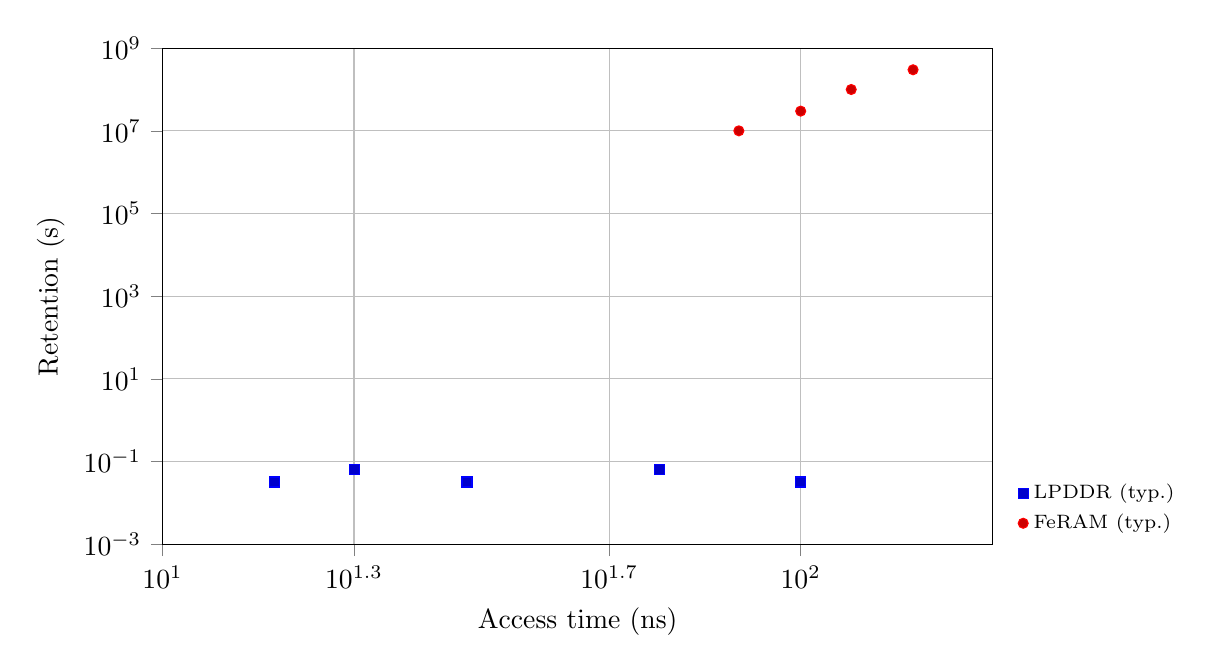
\begin{tikzpicture}
    \begin{loglogaxis}[
      width=\columnwidth,
      height=0.65\columnwidth,
      xlabel={Access time (ns)},
      ylabel={Retention (s)},
      legend style={at={(1.02,0)},anchor=south west, draw=none, fill=white, font=\scriptsize}, % ← 外側
      legend cell align=left,
      grid=both,
      tick align=outside,
      tickpos=left,
      xmin=10, xmax=200,
      ymin=1e-3, ymax=1e9,
      ytickten={-3,-1,1,3,5,7,9},
      xtickten={1,1.3,1.7,2},
      clip=false % ← 凡例が外に出る時の保険
    ]

    % LPDDR
    \addplot+[only marks, mark=square*, mark size=1.8pt]
    coordinates {(15,3.2e-2) (20,6.4e-2) (30,3.2e-2) (60,6.4e-2) (100,3.2e-2)};
    \addlegendentry{LPDDR (typ.)}

    % FeRAM
    \addplot+[only marks, mark=*, mark size=1.8pt]
    coordinates {(80,1.0e7) (100,3.0e7) (120,1.0e8) (150,3.0e8)};
    \addlegendentry{FeRAM (typ.)}

    \end{loglogaxis}
  \end{tikzpicture}
  \vspace{-0.6em}
  \caption{Access time vs.\ retention.}
  \label{fig:access_retention_lpddr_feram}
\end{figure}


\subsection{FeRAM Device and Process}
Ferroelectric RAM (FeRAM) based on doped HfO$_2$ leverages polarization switching to store data with low write voltage and fast access~\cite{MullerAPL2011,KimIEDM2021,NohedaNRM2023}.
Process-wise, FeRAM/FeFET flows require \emph{low-to-mid} temperature stabilization ($\sim$350--450$^\circ$C) to preserve the ferroelectric orthorhombic phase in HfZrO$_2$.

\subsection{Why Monolithic Co-Integration Is Impractical}
LPDDR DRAM arrays rely on high-temperature anneals ($>$700$^\circ$C) to realize high-quality storage capacitors.
Such thermal budgets collapse the ferroelectric phase of HfO$_2$, whereas post-FeRAM low-temperature windows cannot support DRAM capacitor quality.
Therefore, monolithic LPDDR+FeRAM co-fabrication is \textbf{impractical}; a package-level approach is required.

\subsection{Package-Level Integration: Chiplet/SiP/PoP}
Figure~\ref{fig:package_lpddr_feram} shows our organization:
(1) LPDDR remains as a standard DRAM die/package optimized in its own process;
(2) a small FeRAM die (chiplet) is co-packaged on a common substrate (SiP/interposer or PoP);
(3) the SoC connects to both through short, low-parasitic interconnects.
This separation preserves each technology's process window while enabling system-level policies to exploit non-volatility.

% --- Fig.3: パッケージ統合 ---
% ==== Fig. 3: Package cross-section (LPDDR+FeRAM Chiplet Integration) ====
\begin{figure}[t]
  \centering
  \begin{tikzpicture}[node distance=1.2cm, font=\small]

    % CPU/Controller
    \node[draw, thick, minimum width=2.8cm, minimum height=1.0cm, fill=gray!15] (cpu) {CPU / Controller};

    % LPDDR chip
    \node[draw, thick, minimum width=2.8cm, minimum height=1.0cm, fill=gray!15, below=of cpu] (lpddr) {LPDDR DRAM Chip};

    % FeRAM chiplet
    \node[draw, thick, minimum width=2.8cm, minimum height=1.0cm, fill=gray!15, right=3.0cm of lpddr] (feram) {FeRAM Chiplet};

    % SystemDK box (supervision layer)
    \node[draw, thick, dashed, minimum width=8.0cm, minimum height=3.2cm, fit=(cpu) (lpddr) (feram)] (systemdk) {};

    \node[above right=-0.3cm and -0.3cm of systemdk.north west, anchor=north west, font=\small\itshape] 
      {SystemDK Co-Design Supervision};

    % Arrows
    \draw[->, thick] (cpu.south) -- (lpddr.north) node[midway,left] {high bandwidth};
    \draw[->, thick] (cpu.east) -- (feram.west) node[midway,above] {checkpoint / state};
    \draw[<->, thick, dashed] (lpddr.east) -- (feram.south west) node[midway,below] {refresh offloading};

    % Substrate
    \node[draw, thick, fill=gray!10, minimum width=9.0cm, minimum height=0.45cm, below=1.2cm of lpddr.south east, anchor=north east] (substrate) {};
    \node at (substrate) {Package Substrate / Interposer (SiP/PoP)};
    
  \end{tikzpicture}
  \vspace{-1ex}
  \caption{Package-level integration of LPDDR and FeRAM chiplet under SystemDK supervision. LPDDR serves as main working memory, while FeRAM provides checkpointing and refresh suppression via a common substrate (SiP/PoP).}
  \label{fig:package_lpddr_feram}
\end{figure}


\subsection{Interface and Policy Hooks}
The FeRAM chiplet exposes a narrow, reliable link (e.g., mailbox DMA or AXI-lite) for:
\begin{itemize}
  \item \textbf{Checkpoint Write/Read}: bulk DMA of model/activation checkpoints and OS state.
  \item \textbf{Refresh Offloading}: firmware migrates cold regions from LPDDR to FeRAM, suppressing refresh traffic.
  \item \textbf{Instant Resume}: fast restore path avoiding full DRAM warm-up.
\end{itemize}
These hooks are orchestrated by the \emph{SystemDK} co-design framework (policies spanning architecture, package, and OS).

\subsection{Key Technology Parameters}
Table~\ref{tab:tech_params} summarizes representative parameters used by our analysis (also reflected in Fig.~\ref{fig:access_retention_lpddr_feram}).
Values are typical-order estimates for policy exploration; silicon-specific tuning is straightforward.

\begin{table}[t]
  \centering
  \caption{Representative parameters for LPDDR and FeRAM used in evaluation.}
  \label{tab:tech_params}
  \vspace{2pt}
  \small
  \setlength{\tabcolsep}{5pt}
  \begin{tabular}{@{}lcc@{}}
    \toprule
    Parameter & LPDDR (typ.) & FeRAM (typ.) \\
    \midrule
    Access latency & 15--60~ns & 80--150~ns \\
    Retention & volatile (32--64~ms refresh) & years ($10^7$--$10^8$~s) \\
    Write energy/bit & moderate & low \\
    Endurance & $>$10$^{15}$ accesses & 10$^8$--10$^{12}$ writes \\
    Process temp. & caps anneal $>$700$^\circ$C & 350--450$^\circ$C \\
    Role & working memory & checkpoint/state \\
    \bottomrule
  \end{tabular}
\end{table}
